\section{结构设计}
\vspace{1em}
\centerline{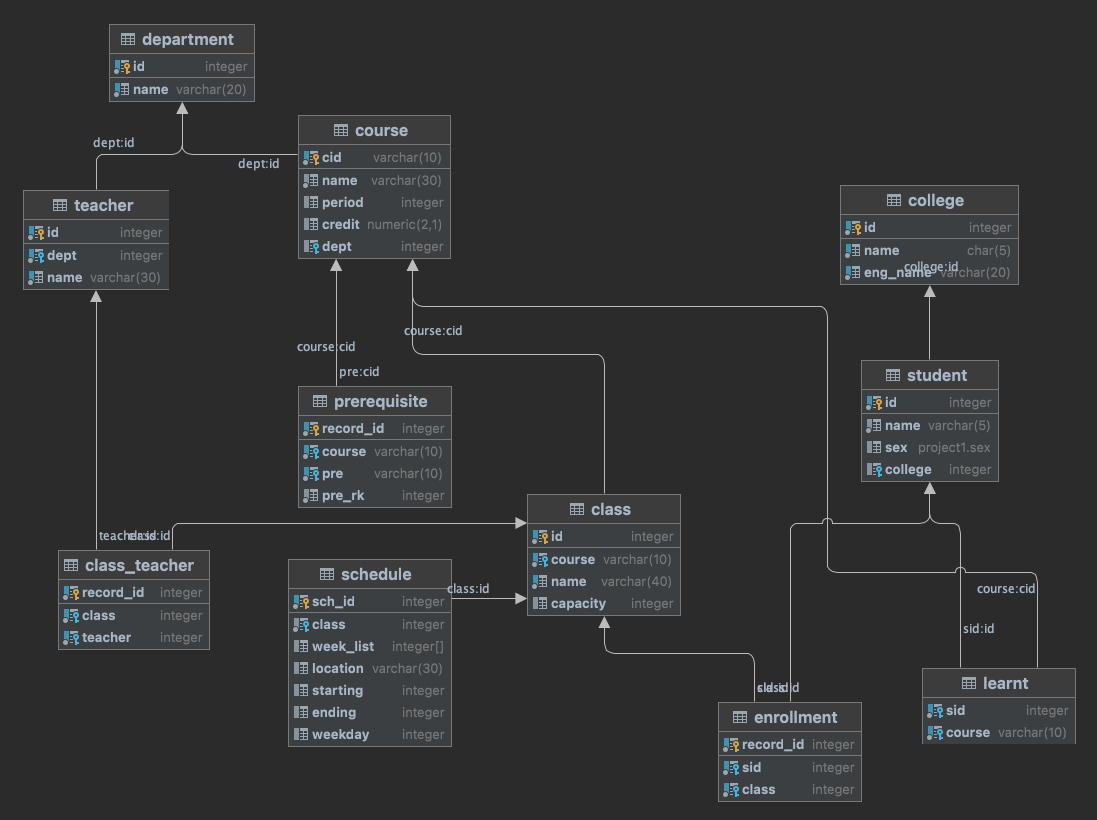
\includegraphics[width=0.9\textwidth]{./pic/ddl.png}}

\subsection{Department}
\begin{lstlisting}
CREATE TABLE department (
    id   serial PRIMARY KEY,
    name varchar(20) UNIQUE NOT NULL
);
\end{lstlisting}
\vspace{-3em}\par
无名的部门是无意义的,故为其加上非空约束,学校中的部门均不重名,即UNIQUE(name)。同时,此表有助于我们减少数据冗余、更方便进行部门更名或删除等操作,也允许了无成员的部门存在。
%Since there's no reason to store a department in each course's info (2NF) and teachers are belonged to departments, we store the information of departments in a table, we can easily add or change info by altering this table. Considering each department in a university surely has a unique name, and there's no reason to store a record with null name, there I put a UNIQUE NOT NULL constraint.

\subsection{Teacher}
\begin{lstlisting}
CREATE TABLE teacher (
    id   serial PRIMARY KEY,
    dept int         NOT NULL REFERENCES department (id),
    name varchar(30) NOT NULL,
    CONSTRAINT teacher_unk UNIQUE (dept, name)
);

\end{lstlisting}
\vspace{-3em}\par
%Each teacher belongs to a department, and it's possible that there exists several teachers in a university sharing the same name, but it's much less possible for it to happen in a single department, and we have no better way to recoginze this unless the data marks it, hence I assert the constraint \emph{name\_unk}.
考虑到学校中可能有重名的教师,而将范围缩小到一个院系里,出现重名的概率大大减少,在无明确指示的情况下我们可以认为部门一致、姓名一致即为同一个人。

\subsection{Course}
\begin{lstlisting}
CREATE TABLE course (
    cid    varchar(10) PRIMARY KEY,
    name   varchar(30) NOT NULL,
    period int CHECK (period > 0),
    credit numeric(2, 1) CHECK (credit >= 0),
    dept   int REFERENCES department (id)
);

\end{lstlisting}
\vspace{-3em}
\par
%This table stores courses like CS201 that may has multiple classes like Bilingual Class 1, 2 and 3. For these classes, they share the same syllabus thus we can aggregate course number \emph{cid}, course name, period, credit and dept into this level. For a course, its course number and name are critical and thus are not null, we can also check the validity of period and credit. Moreover, although there are differences between using int and varchar as primary key\textsuperscript{\cite{pk}}, considering the data volume, frequency of operations and complexity of query statements for later table calls, etc., I kept using course number as the primary key.
本项目共设计三个层次:\emph{course}(共享同一教学大纲)$\to$ \emph{class}(一门课程的多个教学班)$\to$ \emph{schedule}(某一教学班的上课安排)。与int型主键相比,使用varchar对后续的查询性能影响不大\textsuperscript{\cite{pk}},却更加方便查询,均衡二者考虑,选用课程号作为主键。并为\emph{period}(学时)及\emph{credit}(学分)加上合理的检查,减少数据库在经过多次数据更改后误操作修改为特别异常的可能性。

\subsection{Class}
\begin{lstlisting}
CREATE TABLE class (
    id       serial PRIMARY KEY,
    course   varchar(10) REFERENCES course (cid) NOT NULL,
    name     varchar(40)                         NOT NULL,
    capacity int CHECK (capacity > 0)
);
\end{lstlisting}
\vspace{-3em}\par
这里对课程容量进行检查,但允许其置空。另外,存在同一课程的多个班级同名的情况(FIN204有两个英文班),故不加UNIQUE约束。

\subsection{Class-Teacher}
\begin{lstlisting}
CREATE TABLE class_teacher (
    record_id serial PRIMARY KEY,
    class     int REFERENCES class (id)   NOT NULL,
    teacher   int REFERENCES teacher (id) NOT NULL,
    CONSTRAINT cls_tec_unk UNIQUE (class, teacher)
);
\end{lstlisting}
\vspace{-3em}\par
检查数据我们发现,部分班级缺失教师信息,但有教学班同时有数个教师。为了遵循第一范式,我们需要为某班级的所有教师均插入一条记录,且由实际情况可知这不会造成过度的数据膨胀。相比起在Class表中使用数组存教师,使用此表能更加方便的对教师安排进行调动,且能很方便的查询某门课的所有教师或某教师所教授的所有课程。

\subsection{Schedule}
\begin{lstlisting}
CREATE TABLE schedule (
    sch_id    serial PRIMARY KEY,
    class     int REFERENCES class (id) NOT NULL,
    week_list int[],
    location  varchar(30),
    starting  int CHECK (starting >= 1 AND starting <= 12),
    ending    int CHECK (ending >= 1 AND ending <= 12),
    weekday   int CHECK (weekday >= 1 AND weekday <= 7),
    CONSTRAINT time_valid CHECK (ending >= starting)
);
\end{lstlisting}
\vspace{-3em}\par
我们可以为课程时间进行细致的检查(如上四处CHECK所示),另外,考虑到周数列表往往平均长度超过10,若一昧追求1NF,表中将会存入超过教学班数目十倍的记录,且不便于删除,因此将其保存为数组,这样亦能很方便的检查、调整上课周数。

\subsection{Prerequisite}
\begin{lstlisting}
CREATE TABLE prerequisite (
    record_id serial PRIMARY KEY,
    course    varchar(10) REFERENCES course (cid) NOT NULL,
    pre       varchar(10) REFERENCES course (cid) NOT NULL,
    pre_rk    int                                 NOT NULL,
    CONSTRAINT preq_unk UNIQUE (course, pre)
);
\end{lstlisting}
\vspace{-3em}\par
课程的先修要求往往是$(A_1\lor \cdots A_n)\land \cdots \land (Z_1\lor\cdots\lor Z_n)$的形式,一般可将其先以“并且”分割为数块以“或者”链接的子关系。此时我们将“或块”分别标记为\emph{rank},每个rank中只需已学n一门课,且满足所有rank均学过即可。

\subsection{College}
\begin{lstlisting}
CREATE TABLE college (
    id       serial PRIMARY KEY,
    name     char(5) UNIQUE     NOT NULL,
    eng_name varchar(20) UNIQUE NOT NULL
);
\end{lstlisting}
\vspace{-3em}\par
存学生书院信息,这里将中英文名分别存放,并认为学校中所有书院的中、英文名均不相同。

\subsection{Student}
\begin{lstlisting}
CREATE TYPE sex AS enum ('M','F');

CREATE TABLE student (
    id      serial PRIMARY KEY,
    name    varchar(5) NOT NULL,
    sex     sex,
    college int REFERENCES college (id) DEFERRABLE
);
\end{lstlisting}
\vspace{-3em}\par
要保存一条学生记录应该至少知道学生姓名,故将name条目设为非空约束,而其余条目非关键信息可以为空;为了体现要求中"Use appropriate types for different fields of data"且"be as easy to expand as possible",选择用自定义枚举类保存性别,这相比起使用bool标识男女更加直观,且为将来新增性别增加了灵活性。

\subsection{Learnt}
\begin{lstlisting}
CREATE TABLE learnt (
    sid    int REFERENCES student (id) DEFERRABLE NOT NULL,
    course varchar(10) REFERENCES course (cid)    NOT NULL,
    CONSTRAINT learn_unk UNIQUE (sid, course)
);
\end{lstlisting}
\vspace{-3em}\par
数据中未给出选课具体教学班,从常理推测此应该为已学过课程。且学生-课程同时存在才作为一条有意义的记录,故两者均设为NOT NULL,另外认为修完一门课(无论是一次过还是挂科重修)均只留作一条记录,故加上UNIQUE。

\subsection{Enrollment}
\begin{lstlisting}
CREATE TABLE enrollment (
    record_id serial PRIMARY KEY,
    sid       int REFERENCES student (id) DEFERRABLE NOT NULL,
    class     int REFERENCES class (id)              NOT NULL,
    CONSTRAINT enroll_unk UNIQUE (sid, class)
);
\end{lstlisting}
\vspace{-3em}\par
此表存当前学期选课数据,即在开放选课时经过检查满足先修条件后允许插入,删除一条记录即为退课。在本次项目中此表留空。


\section{导入数据}
%\paragraph{Environment}
%\quad PostgreSQL 13.3\quad CentOS Linux release 7.9.2009 \quad Python 3.7.9\\

\subsection{数据清洗}
课程信息json文件的原始数据中包含大量空字符等无意义信息,也存在大量不遵循第一范式的条目。首先需要进行数据清洗,并将清洗完的数据存为新json文件,方便后面对比文件系统与数据库的性能时可以直接使用。而选课信息格式无需清洗,仅在插入数据库时需要检查是否重复以及有无对应课程。

\begin{lstlisting}[language=python]
import pandas as pd

def clear_data(ori: str, out: str):
    with open(ori) as f:
        cif = pd.read_json(f)

    nif = pd.DataFrame()
    nif['totalCapacity'] = cif['totalCapacity']
    nif['courseId'] = cif['courseId']
    nif['prerequisite'] = [clear_pre(pre) for pre in cif['prerequisite']]
    nif['courseHour'] = cif['courseHour']
    nif['courseCredit'] = cif['courseCredit']
    nif['courseName'] = [clear_str(c) for c in cif['courseName']]
    nif['className'] = [clear_str(c) for c in cif['className']]
    nif['courseDept'] = cif['courseDept']
    nif['teacher'] = [clear_teacher(t) for t in cif['teacher']]
    nif['classList'] = clear_class_list(cif['classList'])

    with open(out, 'w+', encoding='utf-8') as f:
        f.write(nif.to_json(orient='records', force_ascii=False))
\end{lstlisting}

\vspace{-3em}\par
我们使用Pandas来更灵活的管理数据框架,检查数据后发现需要清洗的数据为以下几类:
\paragraph{courseName}首位存在空字符,且全半角使用不统一。我们将数据统一使用半角符号,查询时也将用户输入的查询条件清洗为半角即可。
\begin{lstlisting}[language=python]
def clear_str(s):
    if s is None:
        return None
    return s.strip() \
        .replace('(', '(') \
        .replace(')', ')') \
        .replace(',', ',')
\end{lstlisting}
\vspace{-3em}
\begin{lstlisting}[language=python]
>>> clear_str('文物精品研究鉴赏  ')
    '文物精品研究鉴赏'
>>> clear_str('高等数学(下)A')
    '高等数学(下)A'
\end{lstlisting}
\vspace{-3em}

\paragraph{teacher}教师列表不仅存在空字符,也不满足第一范式,我们直接将其处理为Python列表。
\begin{lstlisting}[language=python]
def clear_teacher(t):
    if t is None:
        return None
    return [t.strip() for t in clear_str(t).split(',')]
\end{lstlisting}
\vspace{-3em}
\begin{lstlisting}[language=python]
>>> clear_teacher('\t唐珂 ,  汤小菊\n , Alan Turing  , 于仕琪 '))
	['唐珂', '汤小菊', 'Alan Turing', '于仕琪']
\end{lstlisting}
\vspace{-3em}

\paragraph{prerequisite}
首先按“与”关系分割为数个“或”关系簇,再将其分割为单个课程。有些课程存在多种形式,并存在重复的多项,但为了体现DBMS的性能,这里不做处理,由DBMS负责。其难点在于需要清楚逻辑关系的括号,而不能影响到课程名中的括号,否则课程名中带括号或原有括号被删将影响数据库对课程号的匹配。
\begin{lstlisting}[language=python]
def clear_pre(pre):
    if pre is None:
        return None
    return [[ors.strip('() ') + (')' if ors.strip('() ').endswith(('上', '下')) else '')
             for ors in ands.split('或者')]
            for ands in pre.split('并且')]
\end{lstlisting}
\vspace{-3em}
\begin{lstlisting}[language=python]
>>> clear_pre('(高等数学(下)A 或者 高等数学(下) 或者 数学分析II) 并且 (大学物理A(下) 或者 大学物理 B(下) 或者 大学物理A(下)) 并且 (线性代数I-A 或者 线性代数I)')
    [['高等数学(下)A', '高等数学(下)', '数学分析II'], ['大学物理A(下)', '大学物理 B(下)', '大学物理A(下)'], ['线性代数I-A', '线性代数I']]
\end{lstlisting}
\vspace{-3em}

\paragraph{classList}
其内部又分为多个可能需要清洗的项:
\begin{lstlisting}[language=python]
def clear_class_list(df):
    class_list = []
    for cls in df:
        cls_items = []
        for item in cls:
            item_cls = {}
            item_cls.update({'weekList': [int(x) for x in item.get('weekList')]})
            item_cls.update({'location': clear_str(item.get('location'))})
            item_cls.update({'classTime': item.get('classTime')})
            item_cls.update({'weekday': item.get('weekday')})
            cls_items.append(item_cls)
        class_list.append(cls_items)
    return class_list
\end{lstlisting}
\vspace{-1em}
\centerline{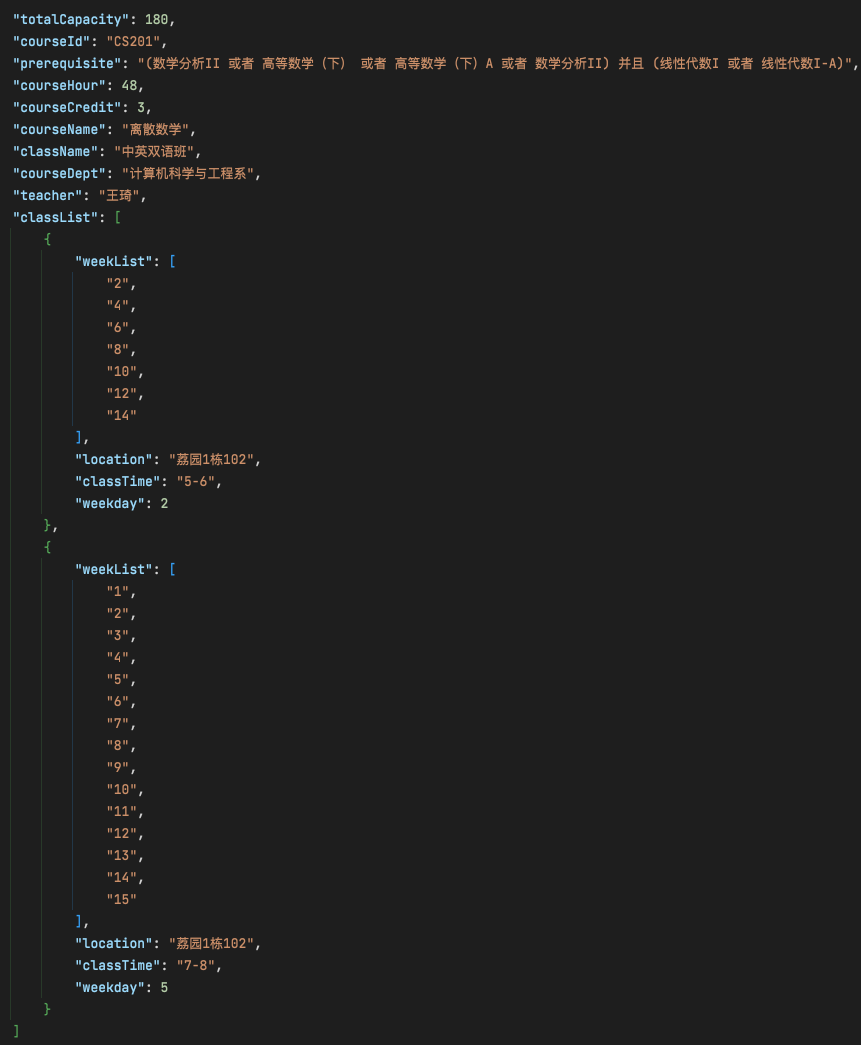
\includegraphics[height=7cm]{dta/clbf.png}\qquad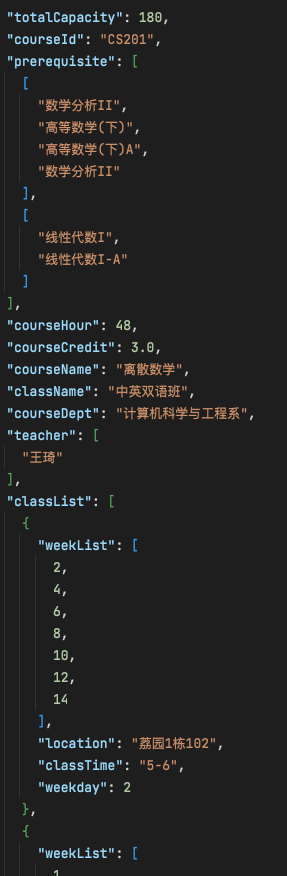
\includegraphics[height=7cm]{dta/claf.png}}
\scriptsize
\centerline{数据清洗前后对比}
\normalsize

\subsection{导入课程信息}
本部分数据量远小于选课数据,因此我们注重于导入的准确性(优化速度的方案于下节展开讨论)。
\par 由于此部分外键限制错综复杂,若只导一次数据,各种子查询及外键冲突处理等会使得DML变得异常复杂且可读性较低,因此,以下我们多次遍历数据,将存在外键约束的条目分别开来。
\begin{lstlisting}[language=python]
import psycopg2 as psql
from psycopg2.extras import execute_batch
# import other packages

class DB:
    def __init__(self, conf: str = './user.yml', data='./data/clear_course_info.json'):
        with open(conf, 'r', encoding='utf-8') as cfg:
            conf = yaml.safe_load(cfg)
        try:
            self.conn = psql.connect(host=conf['host'], port=conf['port'],
                                     user=conf['user'], password=conf['pwd'],
                                     database=conf['db'])
            self.cur = self.conn.cursor()
            self.conn.autocommit = False
        except Exception as e:
            print(e)
            sys.exit(1)
        with open(data, 'r') as dat:
            self.cdata = pd.read_json(dat)
        print('Database connected && Data loaded to RAM.')

    def __del__(self):
        self.conn.commit()
        self.conn.close()
\end{lstlisting}
\vspace{-3em}\par
这里定义了DB类,并在实例化对象时自动连接数据库(连接所需密码、数据库等信息由配置文件读取而得)并将数据载入内存;程序结束销毁对象时进行一次提交并关闭链接。

\begin{lstlisting}[language=python]
def submitter(self, time_start, sql, data):
    print(f'Preparing data in py ({time.perf_counter() - time_start:.4f}s)', end=' >>> ')
    try:
        tm = time.perf_counter()
        execute_batch(self.cur, sql, data)
        self.conn.commit()
        print(f'Submitted {len(data)} requests '
              f'({time.perf_counter() - tm:.4f}s | avg={len(data) / (time.perf_counter() - tm):.4f}i/s)')
    except Exception as e:
        print(e)
\end{lstlisting}
\vspace{-3em}\par
通用提交插入命令的函数,完成了计时,使用批处理(细节于下节讨论)。

\begin{lstlisting}[language=python]
def create_tables(self, ddl_path):
    with open(ddl_path, 'r') as dl:
        sql_list = dl.read().split(';')[:-1]
    try:

        for sql_item in sql_list:
            self.cur.execute(sql_item)
        self.conn.commit()
    except Exception as e:
        print(repr(e))
\end{lstlisting}
\vspace{-3em}\par
为了实现高度的自动化,这里将第一节的DDL及以下两句命令写入SQL文件中。利用PostgreSQL命令由分号结束的性质,此函数逐句执行SQL文件中的命令(删除原有schema并重新建表)。

\begin{lstlisting}
DROP SCHEMA IF EXISTS project1 CASCADE;
CREATE SCHEMA project1;
\end{lstlisting}

\begin{lstlisting}[language=python]
@timer
def ins_dept(self):
    sql = '''
            INSERT INTO project1.department (name)
            VALUES (%s)
            ON CONFLICT DO NOTHING;
          '''
    tm = time.perf_counter()
    dept = [(x,) for x in self.cdata['courseDept']]
    self.submitter(tm, sql, dept)

@timer
def ins_teacher(self):
    sql = '''
            INSERT INTO project1.teacher(name, dept)
            VALUES (%s, (SELECT id
                         FROM project1.department
                         WHERE name = %s))
            ON CONFLICT DO NOTHING;
          '''
    tm = time.perf_counter()
    teacher = []
    for index, item in self.cdata.iterrows():
        if item['teacher'] is None:
            continue
        for t in item['teacher']:
            teacher.append((t, item['courseDept']))
    self.submitter(tm, sql, teacher)

@timer
def ins_course(self):
    sql = '''
            INSERT INTO project1.course
            VALUES (%s, %s, %s, %s, (SELECT id
                                     FROM project1.department
                                     WHERE name = %s))
            ON CONFLICT DO NOTHING;
          '''
    tm = time.perf_counter()
    course = [(item['courseId'], item['courseName'], item['courseHour'],
               item['courseCredit'], item['courseDept'])
              for index, item in self.cdata.iterrows()]
    self.submitter(tm, sql, course)

@timer
def ins_pre(self):
    sql = '''
            WITH preid AS (SELECT cid
                           FROM project1.course
                           WHERE name = %s)
            INSERT INTO project1.prerequisite (course, pre, pre_rk)
                (SELECT %s, (SELECT cid FROM preid LIMIT 1), %s
                 WHERE (SELECT COUNT(cid) FROM preid) > 0)
            ON CONFLICT DO NOTHING;
          '''
    tm = time.perf_counter()
    pres = []
    for index, item in self.cdata.iterrows():
        if item['prerequisite'] is None:
            continue
        for rk, ands in enumerate(item['prerequisite'], start=1):
            for ors in ands:
                pres.append((ors, item['courseId'], rk))
    self.submitter(tm, sql, pres)
\end{lstlisting}
\vspace{-3em}\par
实现避免插入重复一般有两种方案:\ding{172} INSERT INTO <table> (SELECT <values> WHERE (SELECT COUNT(*) FROM <table>) = 0,可见该方法不仅书写复杂,本地为了填充批处理命令也需要准备更多数据;\ding{173} INSERT INTO <table> VALUES (<values>) ON CONFLICT DO NOTHING,不仅书写简单,填充数据少,且DBMS计划任务较简单,执行更快。\\~\\
\centerline{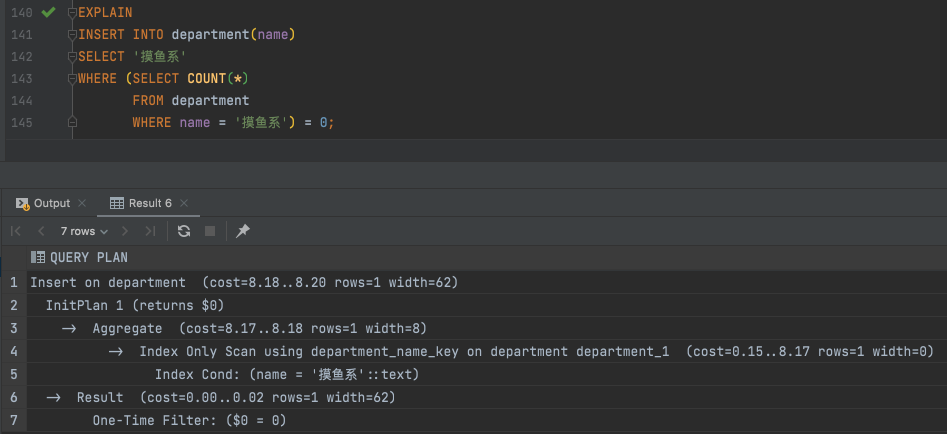
\includegraphics[height=4cm]{dta/ins1.png}\qquad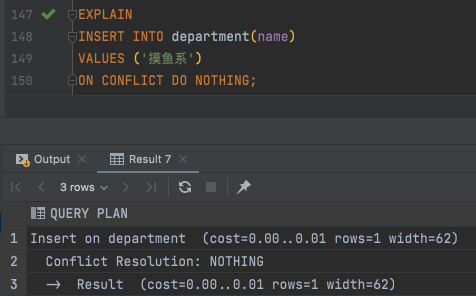
\includegraphics[height=4cm]{dta/ins2.png}}
~\\
\centerline{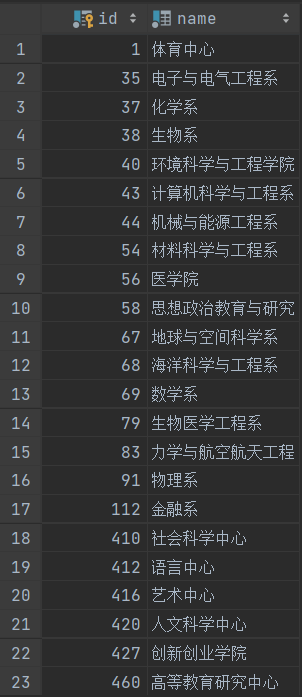
\includegraphics[height=4.5cm]{dta/dept.png}
\quad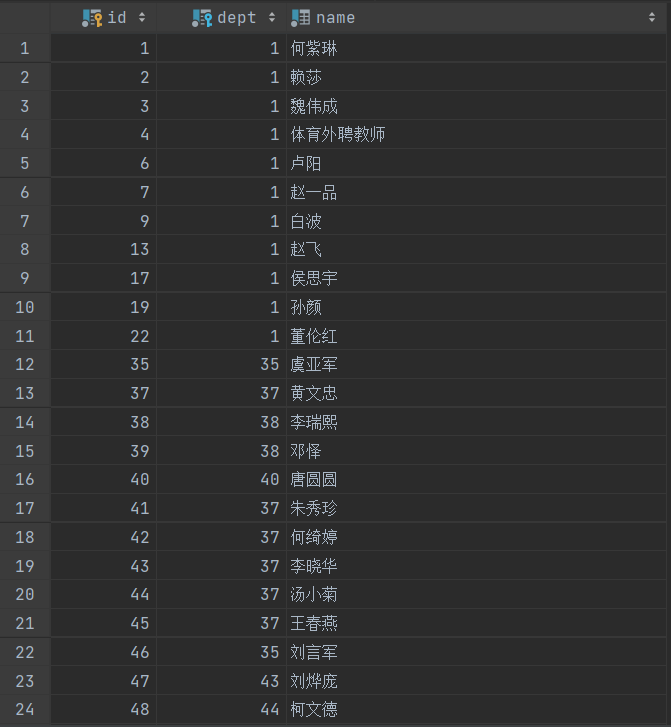
\includegraphics[height=4.5cm]{dta/tech.png}
\quad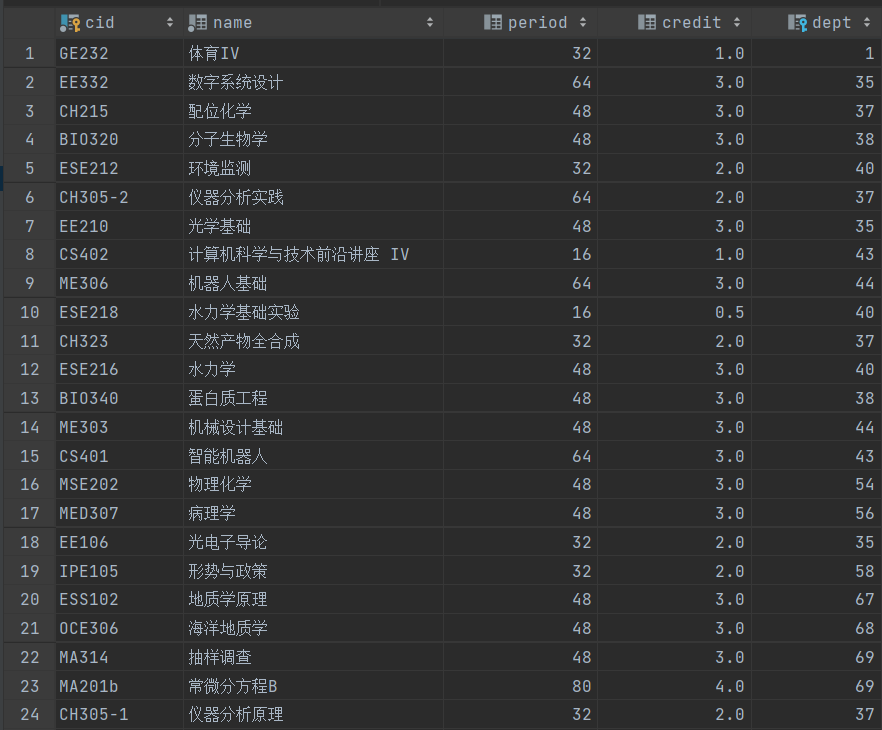
\includegraphics[height=4.5cm]{dta/course.png}
\quad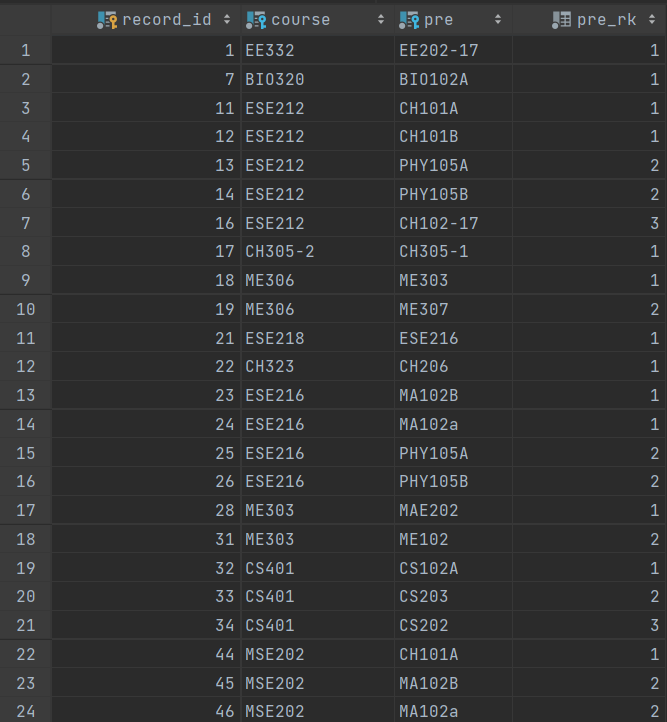
\includegraphics[height=4.5cm]{dta/preq.png}}
\scriptsize\centerline{上示正确插入后的数据存储}\normalsize
~\\

\begin{lstlisting}[language=python]
@timer
def ins_class_te_sc(self):
        sql_cls = '''
                    INSERT INTO project1.class
                    VALUES (%s, %s, %s, %s);
                  '''
        sql_tec = '''
                    WITH tid AS (
                    SELECT id
                    FROM project1.teacher
                    WHERE name = %s
                        AND dept = (SELECT id FROM project1.department WHERE name = %s)
                    )
                    INSERT INTO project1.class_teacher (class, teacher)
                    VALUES (%s, (SELECT id FROM tid));
                  '''
        sql_sch = '''
                    INSERT INTO project1.schedule (class, week_list, location, starting, ending, weekday)
                    VALUES (%s, %s::int[], %s, %s, %s, %s);
                  '''
        tm = time.perf_counter()
        cls = []
        tec = []
        sch = []
        self.cur.execute('''
                           SELECT GREATEST((SELECT last_value - 1
                                            FROM project1.class_id_seq),
                                           (SELECT MAX(id)
                                            FROM project1.class));
                         ''')
        for idx, (index, item) in enumerate(self.cdata.iterrows(), start=self.cur.fetchone()[0] + 1):
            cls.append((idx, item['courseId'], item['className'], item['totalCapacity']))
            if item['teacher'] is not None:
                for x in iter((t, item['courseDept'], idx) for t in item['teacher']):
                    tec.append(x)
            for x in iter((idx,
                           str(cl.get('weekList')).replace('[', '{').replace(']', '}'),
                           cl.get('location'),
                           int(cl.get('classTime').split('-')[0]),
                           int(cl.get('classTime').split('-')[1]),
                           cl.get('weekday'))
                          for cl in item['classList']):
                sch.append(x)
        print(f'Preparing data in py ({time.perf_counter() - tm:.4f}s)', end=' >>> ')
        try:
            tm = time.perf_counter()
            execute_batch(self.cur, sql_cls, cls)
            execute_batch(self.cur, sql_tec, tec)
            execute_batch(self.cur, sql_sch, sch)
            self.cur.execute('SELECT max(id) FROM project1.class')
            self.cur.execute('ALTER SEQUENCE project1.class_id_seq RESTART WITH %s;',
                             self.cur.fetchone()[0] + 1)
            self.conn.commit()
            print(f'Submitted {len(cls) + len(tec) + len(sch)} requests '
                  f'({time.perf_counter() - tm:.4f}s | '
                  f'avg={(len(cls) + len(tec) + len(sch)) / (time.perf_counter() - tm):.4f}i/s)')
        except Exception as e:
            print(e)
\end{lstlisting}
\vspace{-3em}\par
这里我们同时向Class,Class-Teacher和Schedule插入字段。常规的做法是先插入Class,以后在插入Class-Teacher的cid等字段时进行大量的SELECT id操作,显然这非常耗时。考虑到json文件中按教学班存信息,我们可以管理本地index,使得每个Class的index互异且递增(如31行所示),并将相同的index填入此教学班所属的时段和教师。
\par 为了避免主键的UNIQE冲突,我们首先要检测当前表中最大自增ID号及实际存的最大index(在本例中我们知道本地index从1开始即可,但此检测提高了程序的鲁棒性,避免了向非空的表中插入数据时产生的index冲突),并在插入数据后重设DBMS的自增序列(如51行所示),这保证了在以后的插入中如果不指定index,使用自增id不会导致异常。\\~\\
\centerline{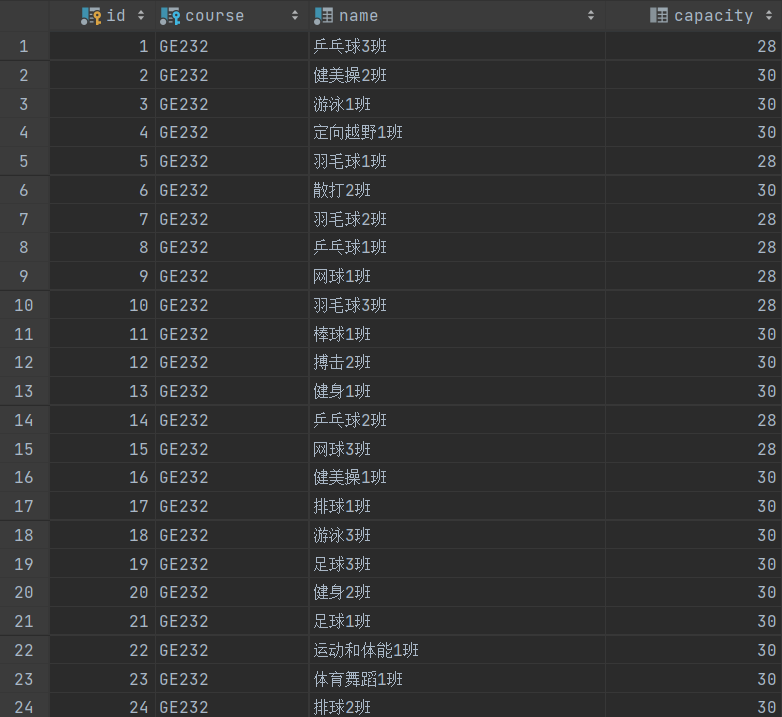
\includegraphics[height=4.2cm]{dta/class.png}\quad
	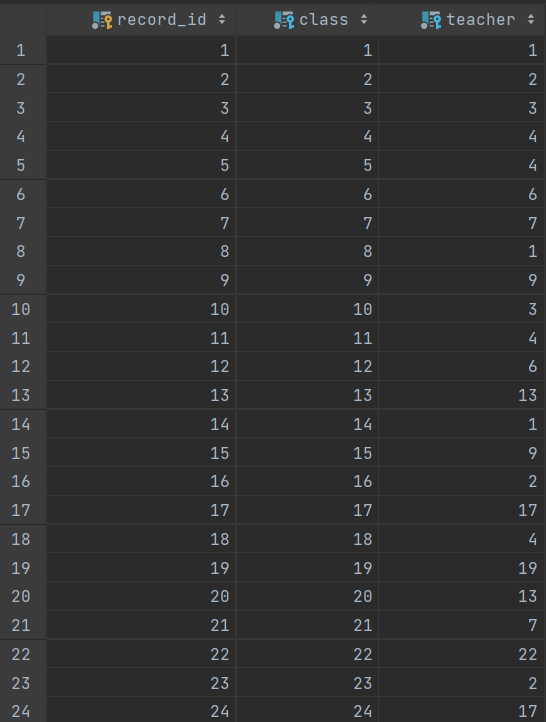
\includegraphics[height=4.2cm]{dta/ct.png}\quad
	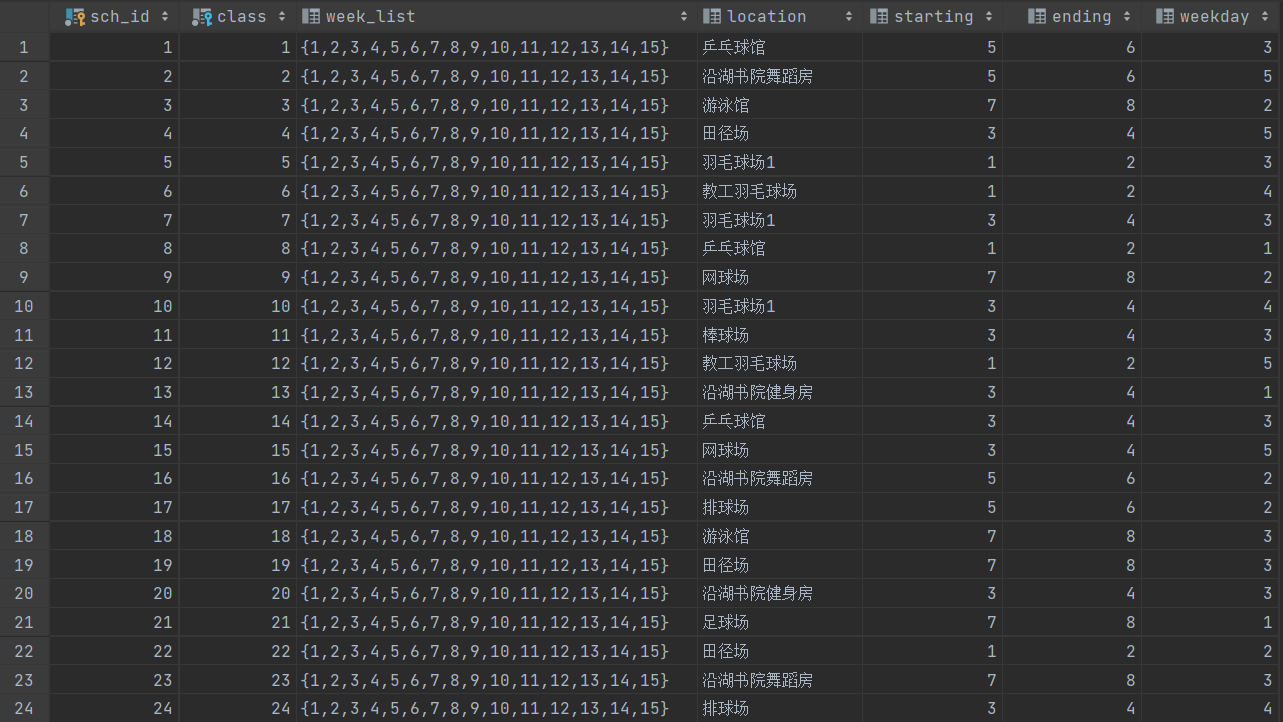
\includegraphics[height=4.2cm]{dta/sch.png}}\\~\\
\centerline{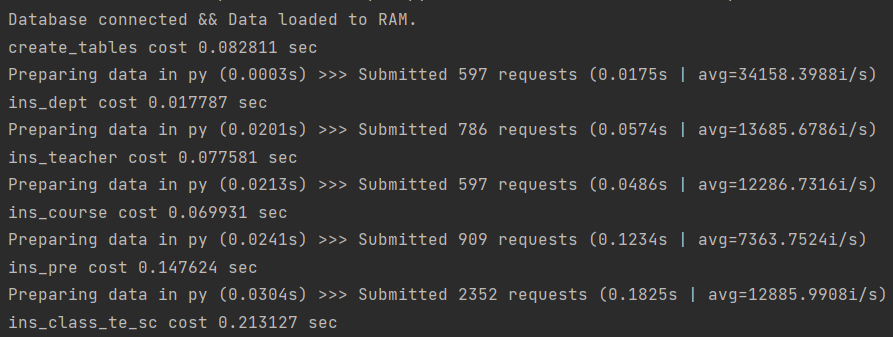
\includegraphics[height=3.5cm]{dta/cisp.png}}
\scriptsize\centerline{插入课程信息平均速度16075 items/sec}\normalsize

\subsection{导入选课信息}
\subsubsection{关闭自动提交}
\begin{lstlisting}[language=python]
@timer
def bad_loader(self):
    for stu in self.cdata:
        try:
            self.cur.execute('''INSERT INTO project1.college(name, eng_name)
                                SELECT %s, %s
                                WHERE (SELECT COUNT(*)
                                       FROM project1.college
                                       WHERE name = %s) = 0;''',
                             (stu[2].split('(')[0],
                              stu[2].split('(')[1].replace(')', ''),
                              stu[2].split('(')[0]))
            self.cur.execute('''INSERT INTO project1.student
                                VALUES (%s, %s, %s, (SELECT id
                                                     FROM project1.college
                                                     WHERE name = %s))
                                ON CONFLICT DO NOTHING;''',
                             (stu[3], stu[0], stu[1], stu[2].split('(')[0]))
            for sel in stu[4:]:
                self.cur.execute('''INSERT INTO project1.learnt
                                    (SELECT %s, %s
                                     WHERE EXISTS(SELECT id FROM project1.student WHERE id = %s)
                                       AND EXISTS(SELECT cid FROM project1.course WHERE cid = %s))
                                     ON CONFLICT DO NOTHING;''',
                                 (stu[3], sel, stu[3], sel))
        except Exception as e:
            print(e)
\end{lstlisting}
\vspace{-3em}\par
需要注意的是psycopg2在建立连接后默认关闭自动提交。实验对比可知相比于autocommit时的插入速度,关闭其将性能提升了约36.7\%。
~\\
\begin{figure*}[!h]
	\centering
	\begin{subfigure}[b]{0.8\textwidth}
		\centerline{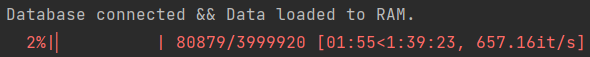
\includegraphics[width=0.6\textwidth]{./sp/autocommit.png}}
		\caption{autocommit = true}
	\end{subfigure}\\
	\begin{subfigure}[b]{0.8\textwidth}
		\centerline{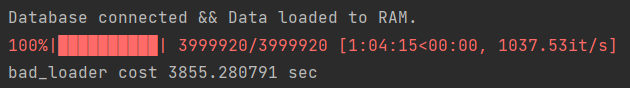
\includegraphics[width=0.6\textwidth]{./sp/bl.png}}
		\caption{autocommit = false, bad\_loader}
	\end{subfigure}	
	\label{fig:visual_smap}
\end{figure*}
\par 分析其原因,自动提交时需要频繁检查数据是否满足ACID,越早插入的数据受越多次检查,从而耗费大量时间;而关闭自动提交大大减少了检测的次数以及每行被检测的平均次数。

\subsubsection{批处理及分页大小}
\begin{lstlisting}[language=python]
@timer
def batch_loader(self, pg: int):
    # prepare data
    try:
        execute_batch(self.cur,
                      '''INSERT INTO project1.college(name, eng_name)
                         SELECT %s, %s
                         ON CONFLICT DO NOTHING;''',
                      college,
                      page_size=pg)
        # similar for student info and course selection
    except Exception as e:
        print(e)
\end{lstlisting}
\vspace{-3em}\par
使用批处理 (psycopg2.extras.execute\_batch) 使得一次操作中可以执行多条SQL语句,相比于一次一次执行效率会提高很多。理论上在一定范围内,batch size (page\_size) 越大,批量操作需要向数据库发送请求的次数越少,速度就越快;以下实验测得当分页大小为1000左右时相较于较小的分页大小有较好的提速效果,但当其进一步加大时(下图(d)),速度反而下降,相较于减少请求次数带来的时间损耗,单次发送请求过大反而降低效果。本项可最多带来约21.7\%的性能提升。
~\\
\begin{figure*}[!h]
	\centering
	\begin{subfigure}[b]{0.8\textwidth}
		\centerline{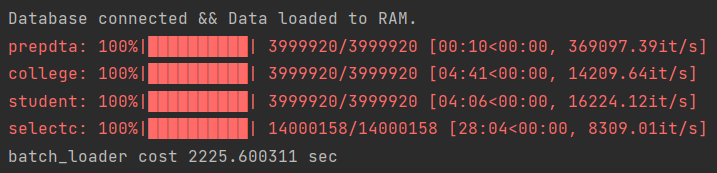
\includegraphics[width=0.6\textwidth]{./sp/batch100.png}}
		\caption{batch size = 100}
	\end{subfigure}\\
	\begin{subfigure}[b]{0.8\textwidth}
		\centerline{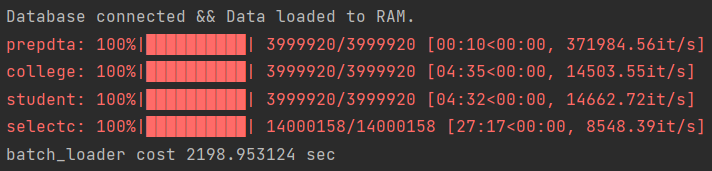
\includegraphics[width=0.6\textwidth]{./sp/batch500.png}}
		\caption{batch size = 500}
	\end{subfigure}	
	\begin{subfigure}[b]{0.8\textwidth}
		\centerline{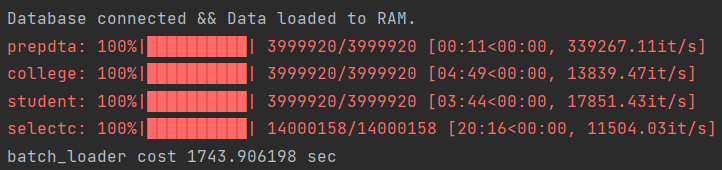
\includegraphics[width=0.6\textwidth]{./sp/batch1000.png}}
		\caption{batch size = 1000}
	\end{subfigure}\\
	\begin{subfigure}[b]{0.8\textwidth}
		\centerline{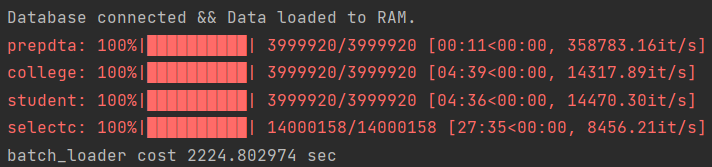
\includegraphics[width=0.6\textwidth]{./sp/batch1500.png}}
		\caption{batch size = 1500}
	\end{subfigure}	
	\label{fig:visual_smap}
\end{figure*}

\subsubsection{延迟检查外键约束}
呼应前面建表中的\emph{deferrable},只需要在batch的基础上加上以下两句就可以在插入事务块中暂时不检查外键约束,而在插入完成后统一检查。
\begin{lstlisting}[language=python]
self.cur.execute('BEGIN TRANSACTION;')
self.cur.execute('SET CONSTRAINTS ALL DEFERRED;')
\end{lstlisting}
\vspace{-3em}\par
如下图所示,尤其是选课数据、学生书院等在插入时能确保满足外键约束的,原来每次插入均花费一定开销检查是否满足外键约束,而延迟检查能节省大量时间。最终用时相比上一步的批处理再次减少46.15\%。\\~\\
\centerline{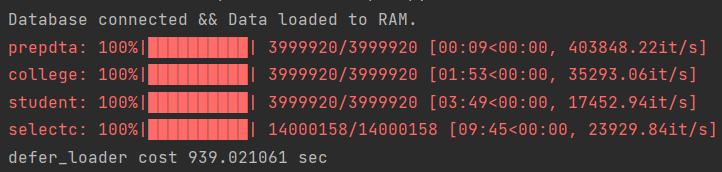
\includegraphics[width=0.6\textwidth]{pic/def.png}}

\subsubsection{异步插入}
\begin{lstlisting}[language=python]
async def async_loader(self):
    with open(conf, 'r', encoding='utf-8') as cfg:
        conf = yaml.safe_load(cfg)
    conn = await asyncpg.connect(host=conf['host'], port=conf['port'],
                                 user=conf['user'], password=conf['pwd'],
                                 database=conf['db'])
    # prepare data
    await conn.execute('BEGIN TRANSACTION;')
    await conn.execute('SET CONSTRAINTS ALL DEFERRED;')
    await conn.executemany('''INSERT INTO project1.college(name, eng_name)
                        	  SELECT $1, $2
                        	  ON CONFLICT DO NOTHING;''', atqdm(college))
    # similar for student info and course selection
    await conn.execute('COMMIT;')
\end{lstlisting}
\vspace{-3em}\par
此时耗时进一步缩短,相比于上一项再次提升约45.15\%,速度达到了平均42718条/秒。然而,异步对于本地数据库提升远不如连接云数据库时带来的提升比例大:如果提供一个网络服务,同时维护很多网络连接,并且每个网络连接都在操作数据库,这个异步过程就非常有意义,它会把数据操作过程本来应该阻塞等待的时间用来处理其它网络连接。\\\vspace{.3em}

\centerline{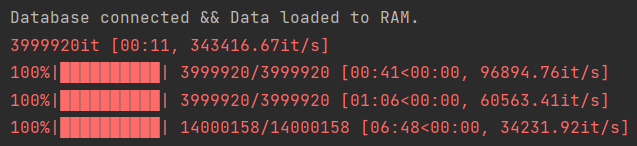
\includegraphics[width=0.6\textwidth]{pic/async.png}}

\subsubsection{连接池}
\begin{lstlisting}[language=python]
async def pool_loader(self, conf='./user.yml'):
    # data
    seq = 0
    for stu in tqdm(self.cdata):
        if seq == 500000:
            seq = 0
            college.append(college_seq.copy())
            stu_info.append(stu_info_seq)
            stu_sel.append(stu_sel_seq)
            college_seq.clear()
            stu_info_seq.clear()
            stu_sel_seq.clear()
        # preparing data packages (500000 students/pkg)
        seq += 1
    college.append(college_seq)
    stu_info.append(stu_info_seq)
    stu_sel.append(stu_sel_seq)
    self.cur.execute('BEGIN TRANSACTION;')
    self.cur.execute('SET CONSTRAINTS ALL DEFERRED;')

    conf = yaml.safe_load(open(conf, 'r', encoding='utf-8'))
    async with asyncpg.create_pool(host=conf['host'], port=conf['port'],
                                   user=conf['user'], password=conf['pwd'],
                                   database=conf['db']) as pool:
        async with pool.acquire() as cur:
            async for seq in atqdm(college):
                await cur.executemany('''INSERT INTO project1.college(name, eng_name)
                                    	 SELECT $1, $2
                                    	 ON CONFLICT DO NOTHING;''', seq)
            # similar for student info and course selection
\end{lstlisting}
\vspace{-3em}\par
在异步插入的基础上应用连接池能进一步提升速度。传统的使用多个连接进行插入会伴随大量的建立、断开连接开销,而上节异步的真正优势体现在高并发或者说并行插入。而连接池实现了连接的复用,正好弥补了上面的缺陷,两者配合,我们将学生数据按50万人/份进行打包,对每个包分别进行批处理插入,综合了以上探究的加速方法的所有优势,最终插入($3999920\times 2+14000158$)条数据总耗时仅216秒,平均每秒插入10.2万条记录,性能约为异步插入的2.38倍。\\\vspace{.3em}

\centerline{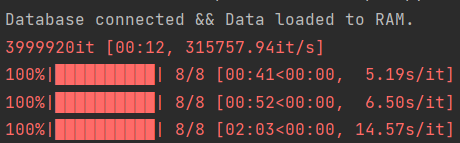
\includegraphics[width=0.4\textwidth]{pic/pkg50w.png}}

下表总结了各方法在插入选课数据(14000158条)时的耗时,由于其数据量较大且DBMS行为统一(无较多的ON CONFLICT DO NOTHING情况),能较好的代表其性能。表中相对提升指应用每项技术相比于不使用所带来的提升,综合性能是此项速度与传统插入的对比。
\begin{table}[H]
\centering
\begin{tabular}{|c|c|c|c|c|c|c|}
\hline
                      & 传统     & 关闭自动提交    & 批处理        & 延迟检查      & 异步插入     & 连接池       \\ \hline
耗时 / s                & 6086   & 3855      & 1216       & 585       & 408      & 123       \\ \hline
速度 / $it\cdot s^{-1}$ & 657.16 & 1037.53   & 11504.03   & 23929.84  & 34231.92 & 113822.42 \\ \hline
相对提升                  & -      & 57.88 \%  & 1008.79 \% & 108.01 \% & 43.05 \% & 232.51 \% \\ \hline
综合性能                  & -      & 157.88 \% & 1750 \%    & 3641 \%   & 5209 \%  & 17320 \%  \\ \hline
\end{tabular}
\end{table}
